\section{How-to}
\subsection{Główne założenia}
Software GS obsługuje się poprzez terminal iPythonowy przez SSH. Najwygodniej jest podzielić obsługę GS na 3 sesje SSH:

\begin{itemize}
	\item Sesja SSH nr 1 - terminal iPythonowy - zbieranie wszystkich odebranych ramek,
	\item Sesja SSH nr 2 - terminal iPythonowy - wykonywanie zadań, sterowanie aktualną sesją komunikacji,
	\item Sesja SSH nr 3 - poruszanie się po komputerze GS, tworzenie katalogów, usuwanie plików, sprawdzanie czy wszystko się zapisało, etc.
\end{itemize}

Aby mieć podgląd na to co leci po radiu w uplinku i downlinku należy połączyć się przez VNC do GS. Aby móc połączyć się do komputera GS przez SSH, czy VNC, musisz być podłączony do PW-Satowego VPN'a. O dane logowania do komputera GS pytaj @mgumiela, @ggajoch, @pkuligowski.

Poniżej przykładowa sesja komunikacji przedstawiona jest na obrazku \ref{fig:gs:samplesession}:
\begin{figure}
	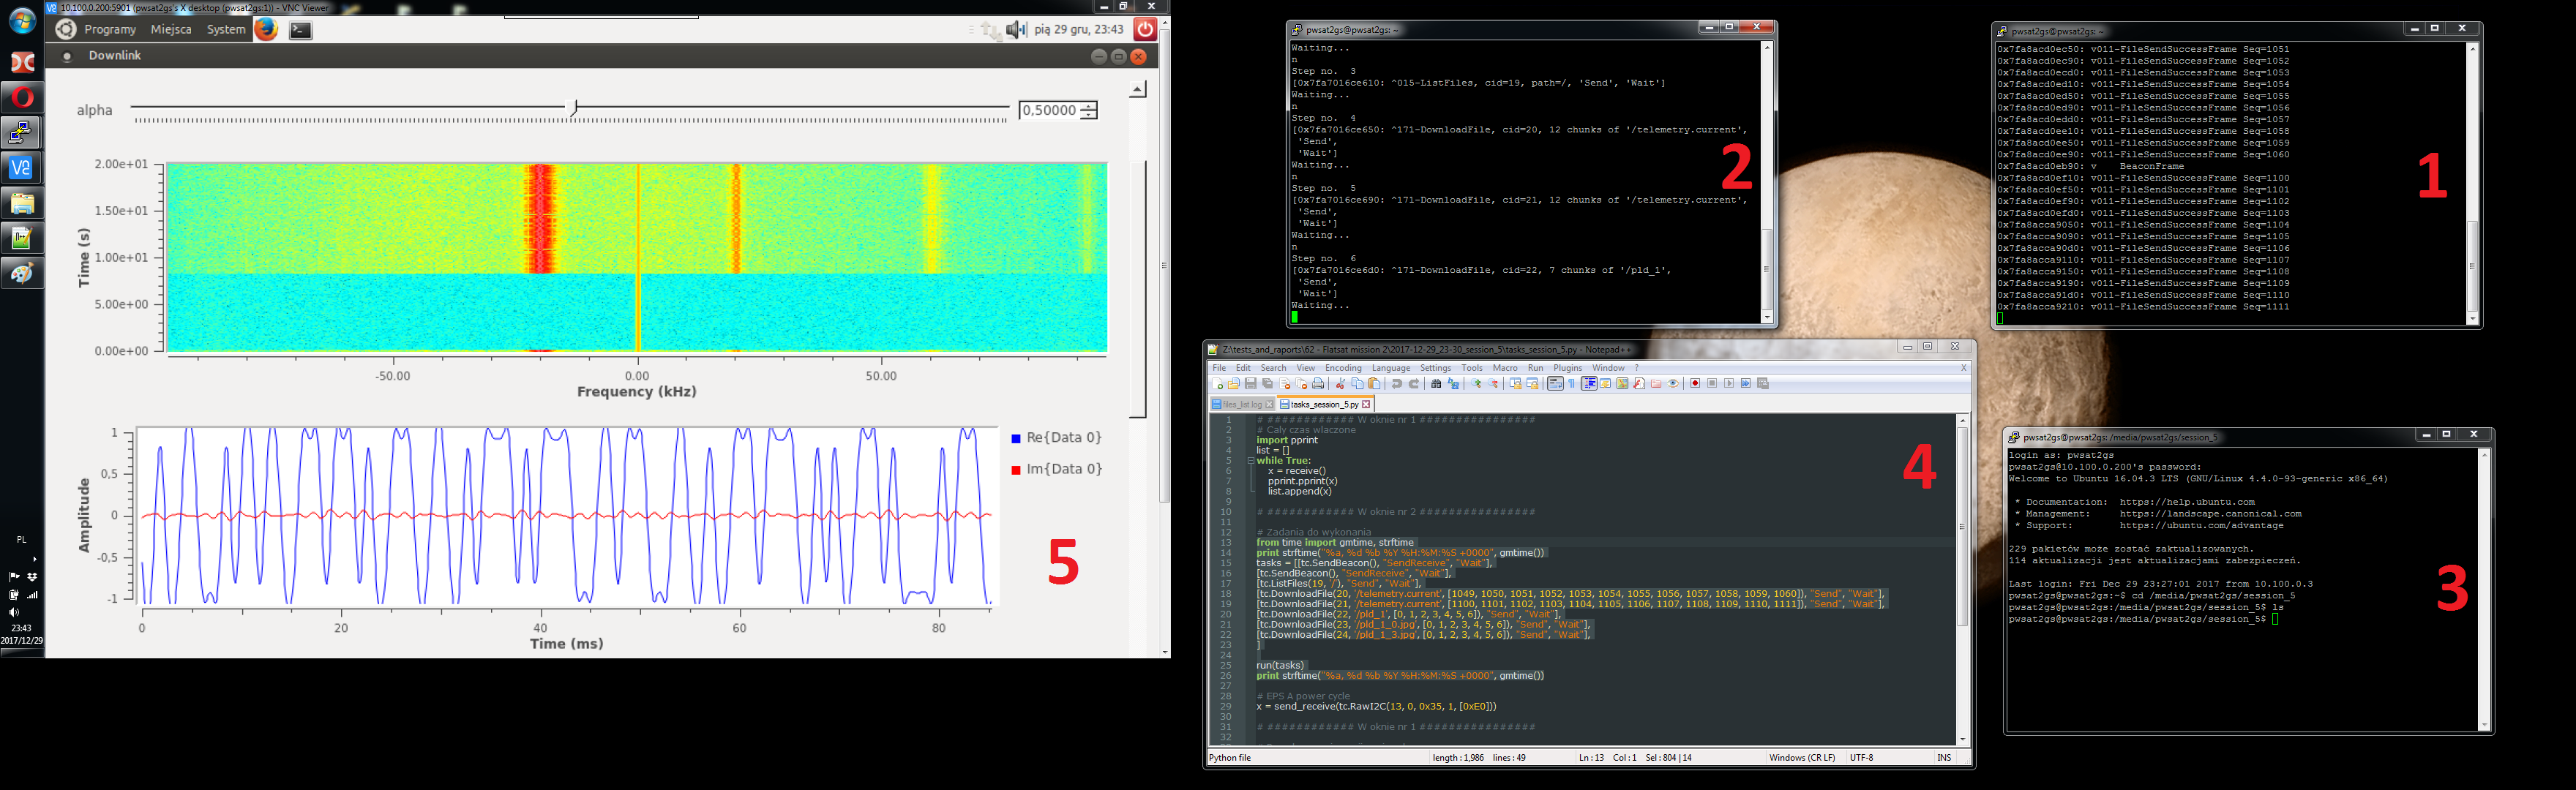
\includegraphics[width=0.8\textwidth]{gs/img/gs-mission-2.png}
	\caption{\label{fig:gs:samplesession} Przykładowa sesja}
\end{figure}

\begin{itemize}
	\item Okno nr 1 - sesja SSH 10.100.0.200:22 nr 1,
	\item Okno nr 2 - sesja SSH 10.100.0.200:22 nr 2,
	\item Okno nr 3 - sesja SSH 10.100.0.200:22 nr 3,
	\item Okno nr 4 - zadania do wykonania w terminalu iPythonowym w oknie nr 2,
	\item Okno nr 5 - sesja VNC 10.100.0.200:5901 z GS - graficzna wizualizacja na to co leci po radiu w uplinku i downlinku. Jeśli aktualnie nie potrzebujesz w cokolwiek klikać, to przełącz się w tryb View-only.
	\item Gdzieś w tle - uruchomiony klient SFTP do pobierania plików z komputera GS.
Potrzebne oprogramowanie:
\end{itemize}

Potrzebne oprogramowanie:
\begin{itemize}
	\item Klient SSH, np. PuTTY,
	\item Klient VNC, np. VNC Viewer,
	\item Klient VPN: OpenVPN,
	\item Klient SFTP: Filezilla/WinSCP.
\end{itemize}

\subsection{Jak to działa na komputerze GS}
Obecnie w GS stoi komputer GS, do którego podłączony jest SDR FUNCube Dongle Pro+ do downlinku i ADALM-PLUTO SDR do uplinku - docelowo uplink musi zostać inaczej rozwiązany. Na komputerze GS jest zainstalowany Ubuntu 16.04.3 LTS wraz z:

\begin{itemize}
	\item GNU Radio - przetwarzanie sygnału z SDR i obsługa SDR,
	\item PW-Sat2 Flatsat Tools - dokładniej podkatalog flatsat_gs z submodułem PWSat2OBC, które obsługują logikę komunikacji, zbierają ramki, zapisują do plików, etc.
	\item PW-Sat2 GS Modem - moduły dla GNU Radio.
	\item PW-Sat2 gr-kiss - fork gr-kiss z wprowadzonymi modyfikacjami na potrzeby PW-Sat2 - do GNU Radio.
\end{itemize}

\subsubsection{GNU Radio}
Na komputerze GS uruchomine jest GNU Radio, które służy do uplinku i downlinku. Składają się na to 3 programy:

\begin{itemize}
	\item uplink - waterfall przesuwa się tylko w momencie wysyłania ramki, normalnie jest nieruchomy. Wszystkie ustawienia domyślne są ok. Zamknięcie tego okna powoduje zamknięcie aplikacji uplinku. Przykład na obrazku \ref{fig:gs:uplink}
	\item funcube_source jako interfejs FUNCube <-> ZMQ. Jest to aplikacja z GUI. Nie może być otwarta x 2. Przykład na obrazku \ref{fig:gs:fcd_source}
	\item downlink biorący dane z ZMQ poprzedniego programu. Wszystkie ustawienia domyśle są ok, trzeba tylko manipulować Symbol rate, jeśli zmieniono baudrate na satelicie. Aby działało, musi być uruchomiony program funcube_source. Waterfall cały czas powinien iść. Przykład na obrazku \ref{fig:gs:downlink}
\end{itemize}

\begin{figure}
	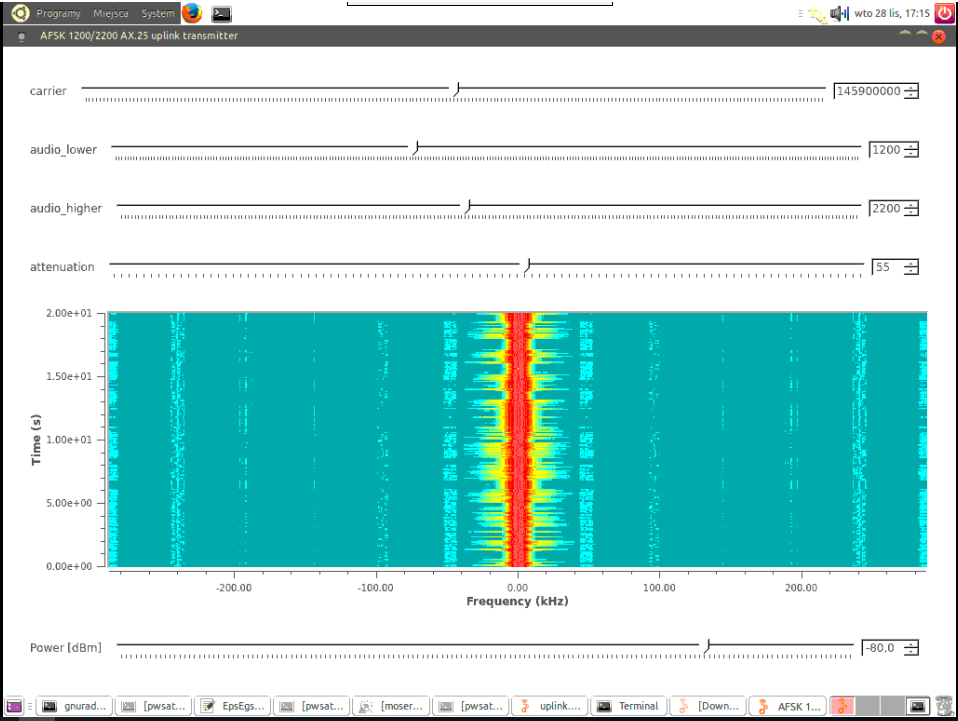
\includegraphics[width=0.8\textwidth]{gs/img/uplink.png}
	\caption{\label{fig:gs:uplink} GNU Radio uplink}
\end{figure}

\begin{figure}
	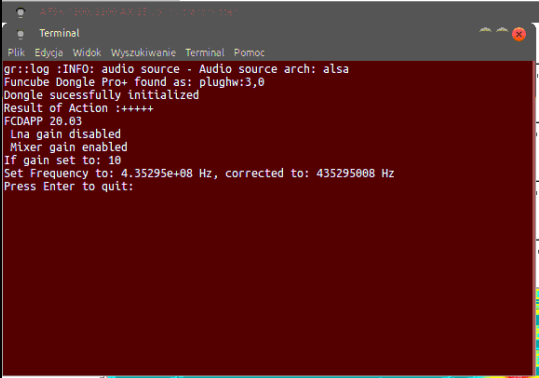
\includegraphics[width=0.8\textwidth]{gs/img/fcd-source.png}
	\caption{\label{fig:gs:fcd_source} FUNcube source}
\end{figure}

\begin{figure}
	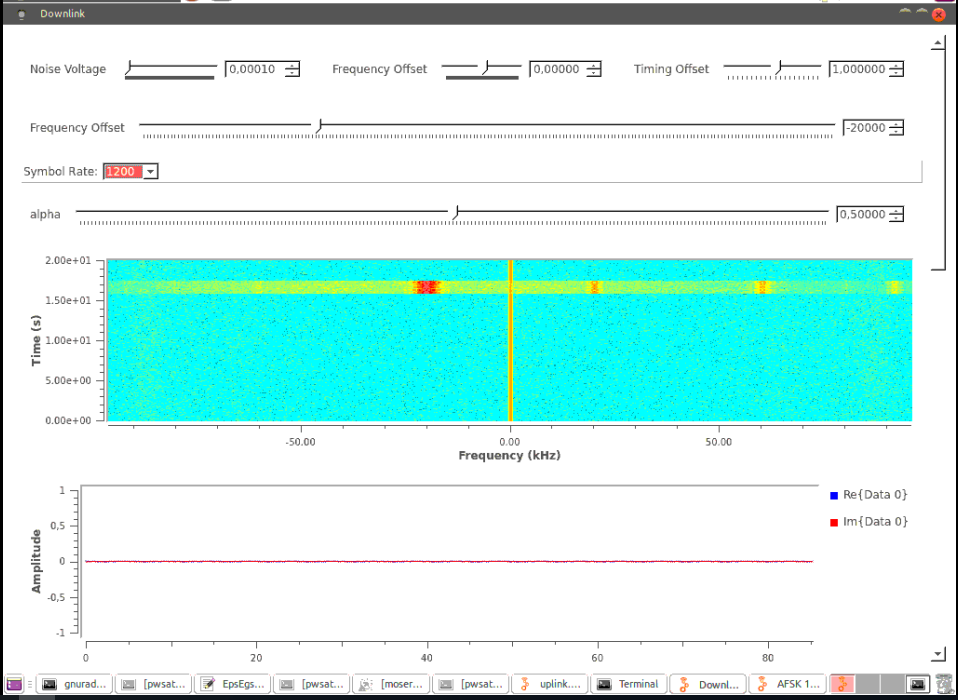
\includegraphics[width=0.8\textwidth]{gs/img/downlink.png}
	\caption{\label{fig:gs:downlink} GNU Radio downlink}
\end{figure}

\subsubsection{W razie awarii}

Uruchamianie GNU Radio:
\begin{lstlisting}[language=bash]
zsh      #<--- koniecznie!
gnuradio-companion
\end{lstlisting}
po uruchomieniu trzeba odpalić każdy z programów, klikając '>'.

\subsection{Terminal iPythonowy}

Do komputera GS należy połączyć się przez SSH. Po nawiązaniu połączenia przez SSH, aby uruchomić terminal iPythonowy w danej sesji SSH, należy wpisać (w jednej linii):

\begin{lstlisting}[language=bash]
sudo python ~/gs/Flatsat-Tools/flatsat_gs/radio/radio_comm.py \
	-c ~/gs/Flatsat-Tools/flatsat_gs/build/integration_tests/config.py}
\end{lstlisting}

\textit{Można mieć uruchomioną dowolną liczbę terminali iPythonowych.}

\subsubsection{Prowadzenie sesji komunikacji}

W jednym terminalu iPythonowym wszystkie odebrane ramki się zbierają (jak to robić - opisane w kolejnym punkcie), a w drugim prowadzona jest sesja komunikacji. Najlepiej jest zaplanować wcześniej co jest do zrobienia i stworzyć gotowy skrypt, który zostanie uruchomiony po złapaniu komunikacji z satelitą. W tym celu należy stworzyć listę pythonową z procedurami do wykonania, która zostanie uruchomiona w terminalu. Przykładowa lista, która powoduje wysłanie telekomend:

\begin{itemize}
	\item ustaw bitrate downlinku na 9600bps - x2,
	\item wyślij beacon - x1,
	\item wyślij listę plików - x1,
	\item wyślij beacon - x4.
\end{itemize}

\begin{lstlisting}[language=Python]
tasks = [[tc.SetBitrate(1, 8), Send, WaitMode.Wait],
	[tc.SetBitrate(2, 8), Send, WaitMode.Wait],
	[tc.SendBeacon(), Send, WaitMode.Wait],
	[tc.ListFiles(3, '/'), Send, WaitMode.Wait],
	[tc.SendBeacon(), Send, WaitMode.Wait],
	[tc.SendBeacon(), Send, WaitMode.Wait],
	[tc.SendBeacon(), Send, WaitMode.Wait],
	[tc.SendBeacon(), Send, WaitMode.Wait],]
}
\end{lstlisting}

W powyższym przypadku parametr Wait powoduje, że po każdej telekomendzie terminal czeka na potwierdzenie, przez wpisanie litery n (jak next) i ENTER. Parametr Send powoduje, że dana linijka tylko wysyła telekomendę, nie czekając na odpowiedź.

Następnie listę tasks można uruchomić w taki sposób:

\begin{lstlisting}[language=Python]
run(tasks)
\end{lstlisting}

Warto notować sobie czas trwania sesji. Można wykorzystać do tego pythona, który wyświetla czas przed i po sesji:

\begin{lstlisting}[language=Python]
import datetime
print datetime.datetime.now().strftime("%Y-%m-%d_%H:%M:%S:%f")
run(tasks)
print datetime.datetime.now().strftime("%Y-%m-%d_%H:%M:%S:%f")
\end{lstlisting}

Można też wysłać pojedynczą telekomendę, bez wpisywania jej w listę:

\begin{lstlisting}[language=Python]
send(tc.SendBeacon())
\end{lstlisting}

Podobnie: wyślij i zwróć pierwszą odebraną ramkę:

\begin{lstlisting}[language=Python]
send_receive(tc.SendBeacon())
\end{lstlisting}

Przydatna automatyka, która requestuje beacona, czeka na niego i parsuje

\begin{lstlisting}[language=Python]
get_beacon()
\end{lstlisting}

Zwraca jedną odebraną ramkę (funkcja blokująca):

\begin{lstlisting}[language=Python]
receive()
\end{lstlisting}

\subsubsection{Odbieranie ramek}
Jeden z terminali iPythonowych powinien być przeznaczony na odbieranie ramek. W tym celu przed sesją komunikacji, należy uruchomić w nim poniższy kod:

\begin{lstlisting}[language=Python]
import pprint
frame_list = []
while True:
x = receive()
pprint.pprint(x)
frame_list.append(x)
\end{lstlisting}

W powyższym skrypcie zastosowano funkcję \lstinline[language=Python]{receive()} zapętloną przez \lstinline[language=Python]{while True:}. Następnie odebrana ramka jest wyświetlana i dodawana do \lstinline{frame_list}.

Po zakończeniu sesji komunikacji skrótem Ctrl+C przerywamy zbieranie ramek. Po tym w obiekcie list zawarta jest lista wszystkich odebranych ramek. Odebrane tak ramki można dowolnie przetwarzać i zapisywać. Najlepiej jest zapisać odebrane ramki ale jeśli się nie uda tego zrobić (np. komputer się zawiesi), to bez paniki: komputer GS loguje wszystkie odebrane ramki i można je odzyskać.

\subsubsection{Zapisywanie odebranych danych}
Mając odebrane ramki w list warto je zapisać/sparsować. Dostępne narzędzia:

\begin{itemize}
	\item \lstinline{RemoteFileTools.parse_file_list(frame_with_list)} - parsowanie listy plików.
	\item \lstinline{save_beacons(path, data)} - parsuje i zapisuje beacony obecne w liście data do pliku path.
	\item \lstinline{parse_and_save(path, data, list_of_correlation_ids)} - parsuje i zapisuje do jednego pliku path ramki FileSuccessFrame obecne w data, takie, które mają \lstinline{correlation_id} zgodne z którymś podanym na liście.
	\item \lstinline{parse_and_save_photo(path, data, list_of_correlation_ids)} - jak wyżej, tylko parsuje jako zdjęcie.
	\item \lstinline{parse_and_save_raw_and_photo(path, data, list_of_correlation_ids)} - dwie powyższe funkcje za jednym razem - uwaga, do 'path` dodaje .raw i .jpg. Poprzednie funkcje nie dodają rozszerzeń.
\end{itemize}